\chapter{Nghiên cứu hệ thống chỉ đường}
\label{Chapter3}

\emph{Chương này sẽ trình bày, mô tả chi tiết về các nghiên cứu đã được thực hiện để giải quyết bài toán chỉ đường, bao gồm danh sách và việc lựa chọn một số thuật toán xử lí giọng nói}

\section{Giới thiệu}
\begin{figure}[htp]
    \centering
    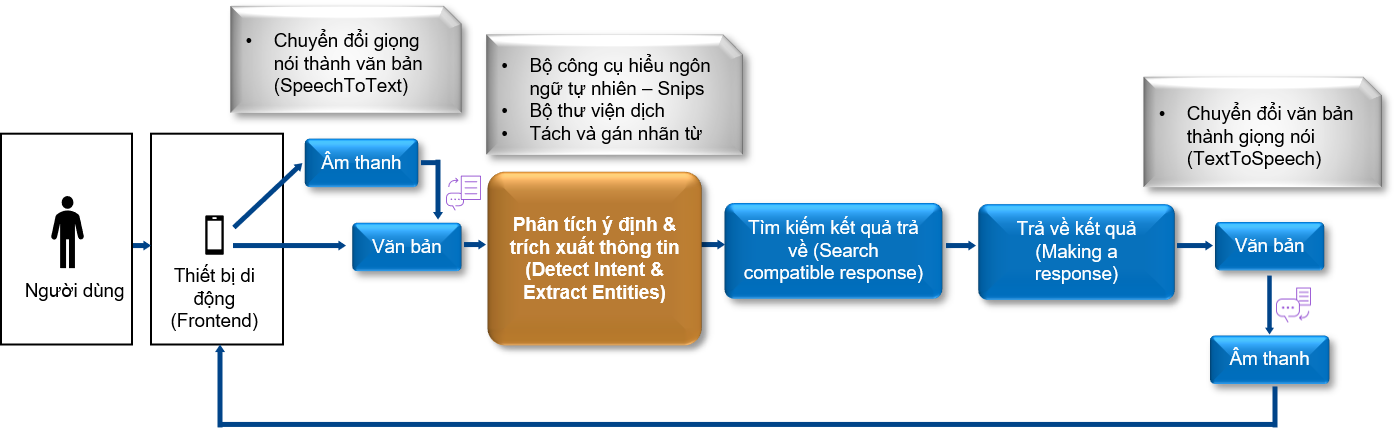
\includegraphics[width=10cm]{images/Structure-description.png}
    \caption{Sơ đồ của hệ thống chỉ đường}
    \label{fig:sodohethongchiduong}

\end{figure}

Khi người dùng sử dụng ứng dụng di động gửi một câu truy vấn bằng audio thì ứng dụng di động sẽ chuyển giọng nói đó thành văn bản (speech to text)

Văn bản đó được gửi tới NLU engine để trích xuất ý định và các thực thể

Dựa trên ý định và thực thể nhận được, hệ thống sẽ truy vấn dữ liệu thông qua google API, tạo ra câu trả lời tương ứng và trả về cho người dùng bằng text và audio ( text to speech để chuyển văn bản thành giọng nói)

Trong phạm vi bài luận này, nhóm em nghiên cứu sử dụng công cụ có sẵn Snips NLU\cite{Snipsnlu} cho việc trích xuất ý định và các thực thể

Snips NLU là công cụ giúp hiểu ngôn ngữ tự nhiên mạnh mẽ, nhưng hiện tại chưa hỗ trợ tiếng Việt, ý tưởng của nhóm em là sẽ tạo một bộ dữ liệu bằng tiếng Việt rồi dịch sang tiếng Anh, dùng dữ liệu tiếng Anh đó để huấn luyện cho mô hình. Khi người dùng truy vấn thì dịch câu truy vấn đó sang tiếng Anh và đưa vào mô hình để trích xuất ý định và các thực thể.

Về mặt dữ liệu:
\begin{itemize}
    \item[--] Định dạng bộ dữ liệu huấn luyện là ở dạng json
    \item[--] Dữ liệu gồm 2 intent là findRoute và askLocation. Mỗi intent gồm 20 câu huấn luyện và 10 câu để kiểm thử
    \item[--] Nhóm em có viết một Script để hỗ trợ việc tạo dữ liệu trở nên đơn dễ dàng hơn.
\end{itemize}

\section{Dịch}

Đầu tiên nhóm em dịch bộ dữ liệu bằng cách tách 1 câu thành từng từ rồi sử dụng thư viện (word2word) để dịch sang tiếng Anh.Vd để dịch câu: "cách đi từ đại học Kinh Tế đến đại học Văn Lang".
\begin{itemize}
    \item[--] Tách câu thành từng từ riêng biệt: ['cách', 'đi', 'từ', 'đại', 'học', 'Kinh' ,'Tế' ,'đến', 'đại', 'học', 'Văn', 'Lang']
    \item[--] Dịch từng từ sang tiếng Anh, ta được: ['ways', 'gone', 'word', 'Swordsman', 'learn', 'GrosDs', 'Monk', 'until', 'Swordsman', 'learn', 'Lam', 'Lang']
\end{itemize}
Sau khi dịch ta được bộ dữ liệu huấn luyện\footnote{Xem thêm về bộ huấn luyện \url{https://drive.google.com/file/d/1yoQk3AuViJpkcDQumQI-SbIw_iGyaGoJ/view?usp=sharing}} và bộ dữ liệu kiểm thử\footnote{Xem thêm về bộ kiểm thử \url{https://drive.google.com/file/d/1i2YNlvZTVsTU2WrzIMBmxl4FcJuAtVyV/view?usp=sharing}}
\begin{figure}[htp]
    \centering
    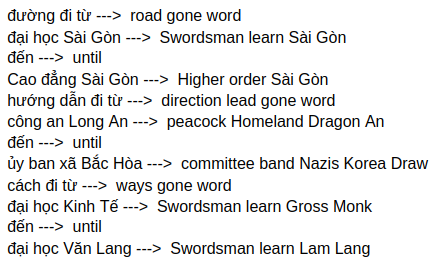
\includegraphics[width=10cm]{images/trainingdata_dichtungtu.png}
    \caption{Hình ảnh minh họa dữ liệu trước khi dịch và sau khi dịch}
    \label{fig:sodohethongchiduong}
\end{figure}

Đem bộ dữ liệu để huấn luyện và đánh giá, ta đạt được kết quả như hình 3.3, xem chi tiết \footnote{\url{https://drive.google.com/file/d/1e2Z0g4irQXqeNMzz4rP1UPQ3OKqYsMPI/view?usp=sharing}}:

\begin{figure}[htp]
    \centering
    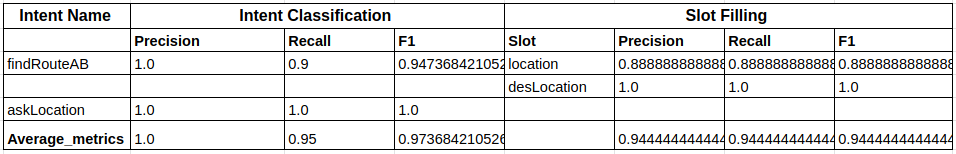
\includegraphics[width=15cm]{images/metrics-dich-tung-t.png}
    \caption{Các chỉ số của mô hình}
    \label{fig:sodohethongchiduong}
\end{figure}
Nhận xét kết quả đạt được:
\begin{itemize}
    \item[--] Mặc dù kết quả tương đối tốt nhưng phương pháp dịch từng từ này không khả thi bởi vì sẽ mà mất ý nghĩa của câu nói, ví dụ như câu sau: "từ Đại học Khoa học Tự nhiên đến Đại học Bách khoa đi như thế nào" được dịch thành "word Swordsman learn department learn itself course until Swordsman learn centurion department" Các thực thể địa điểm như "Đại học Khoa học Tự nhiên" được dịch thành "Swordsman learn department learn itself course", "Đại học Bách khoa" dịch thành "Swordsman learn centurion department"
    \item[--] Các thực thể cần được trích xuất đã bị dịch ra và không còn ý nghĩa nữa, không thể dùng để tìm kiếm địa điểm này trên Google map được.
\end{itemize}

Để xử lý vấn đề này, nhóm em sẽ thay đổi phương pháp dịch bằng cách sử dụng thư viện để tách từ (word segmentation) và gán nhãn từ loại (pos tagging)

Trong tiếng Việt, dấu cách (space) không được sử dụng như 1 kí hiệu phân tách từ, nó chỉ có ý nghĩa phân tách các âm tiết với nhau. Do đó việc tách từ sẽ giúp cho việc dịch được chính xác hơn

Về vấn đề những slot bị dịch thành tiếng Anh làm cho nó không còn ý nghĩa nữa, nhóm em nhận thấy rằng những slot này chủ yếu là danh từ, nên nhóm sẽ sử dụng pos tagging để gán nhãn từ loại, những từ nào thuộc danh từ thì sẽ không cho dịch thành tiếng Anh.

Áp dụng word segmentation và pos tagging lên bộ dữ liệu và sử dụng thư viện word2word để dịch thì đạt được bộ dữ liệu huấn luyện\footnote{\url{https://drive.google.com/file/d/1riZLV1dam9U6q5fuutBFZkzpC6IGgvbb/view?usp=sharing}} và bộ dữ iệu kiểm thử\footnote{	\url{https://drive.google.com/file/d/1Jq1x3-owrcL1TN1igPr7HFNRxTk2emW2/view?usp=sharing}
}:
\begin{figure}[htp]
    \centering
    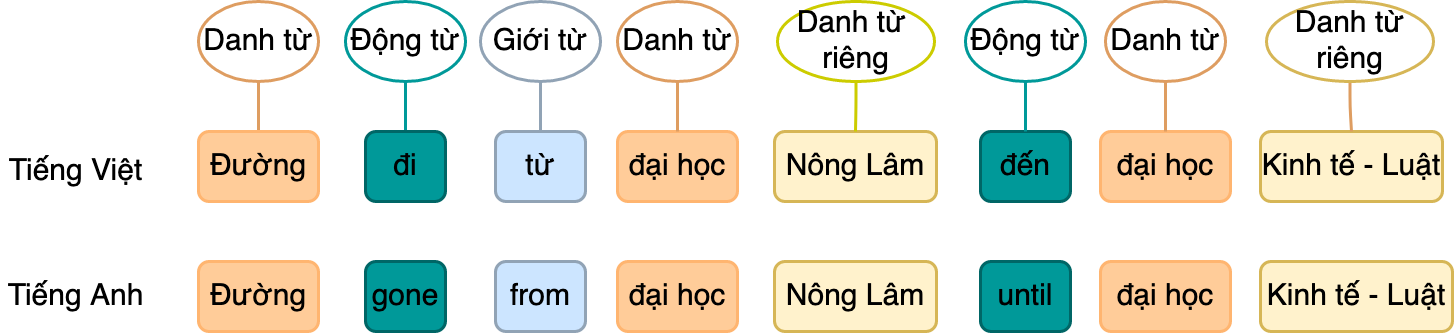
\includegraphics[width=10cm]{images/trainingdata-wordsegment.png}
    \caption{Hình ảnh minh họa dữ liệu trước khi dịch và sau khi dịch bằng phương pháp dùng word segmentation và pos tagging}
    \label{fig:sodohethongchiduong}
\end{figure}

Sau khi huấn luyện mô hình và đem đi đánh giá nhóm nhận được kết quả như  hình 3.4, xem chi tiết \footnote{\url{https://drive.google.com/file/d/1UU7_04Ps6WHZXSujZxNqaZKZhtvYsnrL/view?usp=sharing}}:

\begin{figure}[htp]
    \centering
    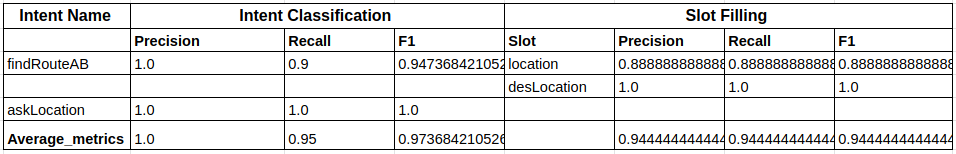
\includegraphics[width=15cm]{images/metrics-dich-tung-t.png}
    \caption{Các chỉ số của mô hình}
    \label{fig:sodohethongchiduong}

\end{figure}

Nhận xét kết quả đạt được:
\begin{itemize}
    \item[--] Sau khi áp dụng tách từ và phân loại từ vựng, nhóm đã xử lý tương đối được vấn đề dịch những slot làm mất ý nghĩa của chúng: "từ Đại học Khoa học Tự nhiên đến Đại học Bách khoa đi như thế nào" được dịch thành "word đại\_học khoa\_học\_tự\_nhiên until đại\_học bách\_khoa gone như\_thế\_nào"
\end{itemize}
Tuy nhiên vẫn còn một vài trường hợp dịch còn chưa ổn, ví dụ như "Đại học Khoa học Xã hội và Nhân văn" được dịch thành "Đại học Khoa học Xã hội their Nhân văn"

Nhóm nhận thấy rằng có thể cải thiện được bộ dịch tốt hơn, nhóm sẽ thay đổi phương pháp dịch bằng cách xây dựng một bộ từ điển, bộ từ điển này nằm trong phạm vi hỏi đường nên có thể xây dựng được, từ đó việc dịch sẽ đạt hiệu quả hơn.

Để cải thiện quá trình dịch từ tiếng Việt sang tiếng Anh, nhóm chúng em đã quyết định xây dựng bộ từ điển riêng để có thể dịch được kết quả chính xác hơn.
Trong phạm vi các câu hỏi về đường đi, chúng em đã lựa chọn dịch khoảng 50 từ và các cụm từ. Các bước để dịch được dữ liệu như sau:
\begin{itemize}
    \item[--] Bước 1: Xây dựng bộ từ điển riêng biệt về chủ đề hỏi đường đi và chuyển hoá từ ngôn ngữ tiếng Việt sang tiếng Anh.
    \item[--] Bước 2: Tìm từ dài nhất trong câu có trong bộ từ điển.
    \item[--] Bước 3: Lấy nghĩa của từ tương ứng trong từ điển.
\end{itemize}
Trong quá trình nghiên cứu, chúng em nhận thấy bước 2 là bước thật sự cần thiết để có thể tìm được từ thích hợp nhất với bộ từ điển để có kết quả tốt nhất. Dưới đây là mô tả quá trình tìm từ dài nhất có trong từ điển mà nhóm chúng em thực hiện (Xem hình Tìm từ dài nhất \ref{fig:longest-word})
\begin{itemize}
    \item[--] Input: "Đường đi từ Đại học Nông Lâm đến Ngã tư Thủ Đức""
    \item[--] Output: ["Đường đi", "từ", "Đại học Nông Lâm", "đến", "Ngã tư Thủ Đức"]
\end{itemize}
\begin{figure}[htp]
    \centering
    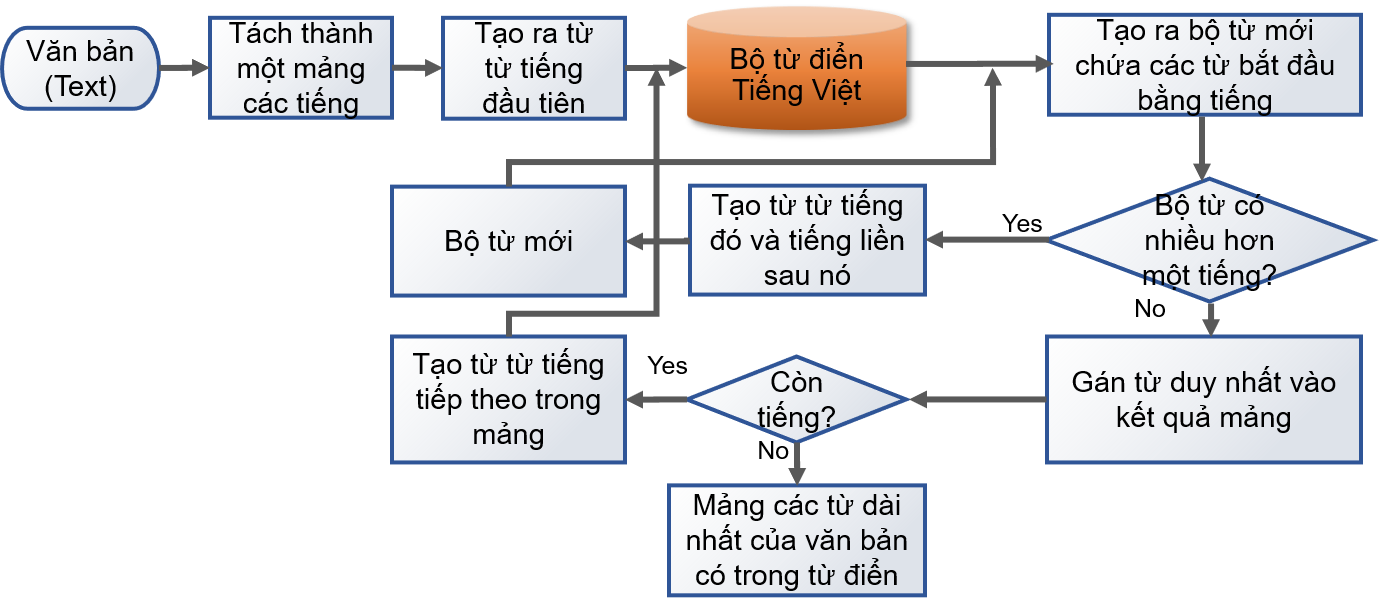
\includegraphics[width=10cm]{images/Diagram-longest-word.png}
    \caption{Tìm từ dài nhất}
    \label{fig:longest-word}
\end{figure}

Sau khi dịch ta được bộ dữ liệu huấn luyện\footnote{\url{https://drive.google.com/file/d/1l6TW8QdhZYOC7uhCpIJpsuSwVfrSv5ie/view?usp=sharing}} và bộ dữ liệu kiểm thử \footnote{\url{https://drive.google.com/file/d/1DpIxFSOjwP_djW-V1jpaLH4HTwGgGZkA/view?usp=sharing}}
\begin{figure}[htp]
    \centering
    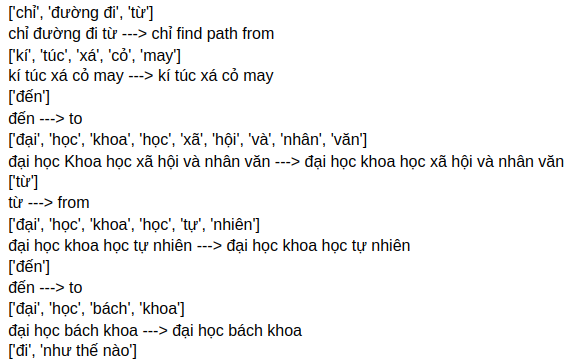
\includegraphics[width=10cm]{images/trainingdata-tudien.png}
    \caption{Hình ảnh minh họa dữ liệu trước khi dịch và sau khi dịch bằng phương pháp xây dựng từ điển}
    \label{fig:sodohethongchiduong}

\end{figure}

Đem bộ dữ liệu để huấn luyện và đánh giá, ta đạt được kết quả như hình 3.8, xem chi tiết \footnote{\url{https://drive.google.com/file/d/1HSe-ri76d8jbF3FZUCrDiFawHI17D18a/view?usp=sharing}}:

\begin{figure}[htp]
    \centering
    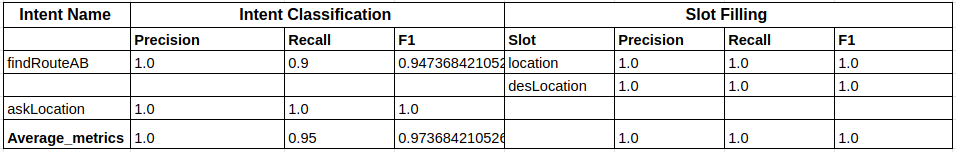
\includegraphics[width=15cm]{images/metrics-tudien.png}
    \caption{Các chỉ số của mô hình}
    \label{fig:sodohethongchiduong}
\end{figure}
Kết quả đạt được sau khi dùng phương pháp dịch bằng cách xây dựng bộ từ điển:
\begin{itemize}
    \item[--] Do xây dựng bộ từ điển những từ vựng trong phạm vi nhỏ - hỏi đường nên bộ dịch cho ra kết quả khá khả quan, cải thiện hơn so với 2 phương pháp trước là phương pháp dịch từng từ và phương pháp dịch dùng word segmentation và pos tagging
    \item[--] Kế hoạch phát triển là xây dựng thêm dữ liệu, tạo thêm nhiều ý định sau đó thực hiện đánh giá mô hình để xem mô hình có thực sự hiệu quả hay không.
\end{itemize}